\documentclass[12pt]{article}


%%%%%%%%%%%%%%%%%%%%%%%%%%%%%%%%%%%%%%%%%%%%%%%%%%%%%%%%%%%%%%%%%%%%%%%%%%%%%%%%%%%%%%
%%%%%%%%%%%%%%%%%%% YOU PROBABLY DON"T NEED TO CHANGE ANYTHING HERE %%%%%%%%%%%%%%%%%%%
\usepackage[numbers,sort]{natbib}
\usepackage{amsfonts, amsmath} 
\usepackage{graphicx}
\usepackage{libertine} 
\usepackage[margin=0.75in]{geometry}
\usepackage{hyperref}
\usepackage{subcaption}
\usepackage{placeins}
\hypersetup{
    colorlinks = true,
    linkcolor = blue,
    urlcolor  = blue,
    citecolor = blue,
    anchorcolor = blue}
\urlstyle{same}
%%%%%%%%%%%%%%%%%%%%%%%%%%%%%%%%%%%%%%%%%%%%%%%%%%%%%%%%%%%%%%%%%%%%%%%%%%%%%%%%%%%%%%
%%%%%%%%%%%%%%%%%%%%%%%%%%%%%%%%%%%%%%%%%%%%%%%%%%%%%%%%%%%%%%%%%%%%%%%%%%%%%%%%%%%%%%


%
% ===== DOCUMENT STARTS HERE =======
% you do not have to modify anything above
% if you do not wish to (but you indeed can)
%
\begin{document}

\title{A Comparison of Baysian Optimisation, TurBO and CMA-ES}
\date{\today}
\maketitle

{\bf Group Composition:}
\begin{enumerate}
\item Lim Zhao Xun Jerrell, A0270410X, e1117759@u.nus.edu
\end{enumerate}

{\bf Github Repository:} \url{https://github.com/JerrellLim/DSA4212-report}

%
\section{Introduction}
Black-box Optimization (BBO) describes a class of optimization problems for which the objective function has no closed form which admits easy evaluation. This could arise either because the objective function is derived from an experiment, the running and re-running of which takes real world monetary cost and time, or due to physical limitations of the experiment apparatus (for instance a machine that breaks down after too many uses). There is also the possibility of noisy evaluations that distort the true observed value of the objective function from the measured value. For this reason, many algorithms for BBO are evaluated not just on accuracy, but the number of evaluations needed to reach the accuracy, as well as how well they handle noisy measurements. In this report, we shall consider 3 BBO algorithms: Bayesian Optimization (BO), a local variant of Bayesian Optimization called TurBO, and 
Matrix Adaptation Evolution Strategy (CMA-ES) and compare their performance on a suite of benchmark functions. We first begin with a review of the 3 BBO algorithms

\subsection{Bayesian Optimization}
The naive BO works by fitting a Gaussian Process (GP) to a collection of functions over some fixed domain $D$. Each evaluation restricts the class of functions that can be consistent with the previous data and conditions this GP. Note that the GP is a global model for the function to be optimized, together with an uncertainty. Given $x \in D$, the mean and variance of $f(x)$ given the conditioned GP informs where the next point should be sampled. This is done through the use of an acquisition function. In our experiments, we consider three such functions, expected improvement (EI), probability of improvement (PI) and Upper Confidence Bound (UCB). More recently, other acquisition functions, like the knowledge gradient (KG) and entropy search (ES) have been developed but we shall omit them from the analysis as their implementation requires one additional loop of simulation to compute enough sample points and approximate the KG or ES. This means each call of the acquisition function becomes too expensive to run. \\

BO is known to perform well in low dimensional settings and with a limited budget (i.e. only making a few evaluations). However, a key assumption in BO is that the underlying BBO is continuous (in the case of ES acquisition a stronger assumption of continuously $C^1$ is required). This is because the kernel functions are often chosen to be continuous (for eg. the exponential kernel), that means for points $x1,x2$ close to each other, $f(x1), f(x2)$ are assumed to be strongly correlated. A hyperparameter learning algorithm can be used to update the parameters in the kernel so that the modulus of continuity becomes larger with more data but then such an algorithm necessarily takes a lot of evaluation before it is able to suitable model a non-continuous objective function.
\subsection{TurBO}
In higher dimensions, large regions of uncertainty may cause the acquisition function to allocate evaluations to areas that are less promising than regions
already identified as having good objective values. The time complexity of fitting a GP also increases with the number of observations, which can become a limitation when a large evaluation budget is available as the algorithm generally takes much longer to converge.\\

One solution is to replace global search with local search. The motivation is that, once a promising region has been identified, it may be more efficient to concentrate evaluations there rather than
continue modeling and searching the entire domain.\\  

However, a purely local search has its own limitations: it may converge to a local minimum without discovering the global minimum, particularly when the objective is multi-modal or the initial point lies in an unpromising region. Trust Region Bayesian Optimization (TuRBO) addresses this limitation by using multiple adaptive-trust regions that can expand and shrink. A local GP is fitted to each trust region and candidate points are generated to guide the selection of subsequent evaluations.
The region is expanded when successive evaluations yield sufficient
improvement and contracted when progress is inadequate. If the region
becomes too small, the algorithm restarts the local search in a new
region.\\ 

In our implementation, we use TurBO-1, which maintains a single trust region at a time and restarts when that region becomes too small. Following the same method as \cite{turboarticle}, the local surrogate is a GP with a Matern $5/2$ kernel, and candidate points are selected using an approximate form of Thompson sampling.

\subsection{CMA-ES}
CMA-ES operates by sampling a population of candidate solutions from a multivariate normal distribution whose mean and covariance are updated at every iteration. This allows the algorithm to automatically handle correlated variables, scaling differences, and arbitrary rotations without requiring explicit gradient information.\\

CMA-ES is widely recognized for its robustness in medium-dimensional settings and excels in rugged, multi-modal, or noisy landscapes where global surrogate models fail \cite{CMA}. Because it relies on the rank-ordering of population members rather than their absolute objective values, it is invariant to monotonic transformations of the objective function. Furthermore, unlike BO, CMA-ES does not suffer from the computational bottlenecks of kernel hyperparameter fitting or strict continuity assumptions, making it well-suited for non-smooth or discontinuous objectives. Most CMA-ES implementations also use an adaptive step-size that scales the covariance matrix to decide how "wide" to cast the net of sampled points. This has the effect of preventing the algorithm from settling into a local valley.\\

However, standard CMA-ES has notable limitations. It typically requires a larger evaluation budget to converge compared to low-budget methods like BO or TuRBO, making it suboptimal when evaluations are extremely expensive. Additionally, the computational complexity of updating and decomposing the full covariance matrix scales quadratically or cubically ($O(N^2)$ to $O(N^3)$) with the problem dimension $N$, which can become a severe bottleneck in very high dimensions unless memory-efficient variants (such as LM-CMA) are employed.

\section{Experiments}
We propose three sets of experiments. The first experiment investigates whether repeated sampling of the same point at the cost of exploring other points helps or hurts the convergence to the true minima in the presence of noise. We consider relatively simple functions (sphere, rastrigin (See formula: \ref{rast formula}) at dimension $d$) with a budget of $50d$ when $d = 5,10$ and $20d$ when $d = 20, 50, 100, 200$. The latter choice of fewer budget is to generate enough data in a timely manner for an accurate statistical comparison. The experiment compares 3 re-evaluation rates ($repeat\_count = 1,2,4$) for BO, CMA, TurBO and a random search for control. The random search looks for the next point to evaluate without reference to any surrogate probability distribution. For this experiment, we look at the objective value returned as well as the time taken to complete the evaluation. For reproducibility, whenever we need to sample from a Gaussian or t-student's noise, the default seed of $2026$ is used.\\

The second experiment aims to compare performance on multi-modal functions. We test three functions
\begin{itemize}
    \label{rast formula} \item Rastrigin: $$f(\mathbf{x}) = 10d + \sum_{i=1}^d \left[x_i^2 - 10\cos(2\pi x_i)\right]$$ which has a global minimum at $0$ and many local minima along the integer lattice points. This tests the ability of an optimization algorithm to escape from local minima. A failure here indicates usually indicates poor step size adaptability. 
    \item Ackley: \[f(\mathbf{x}) =-20\exp\left(-0.2\sqrt{\frac{1}{d}\sum_{i=1}^{d}x_i^2}\right)-\exp\left(\frac{1}{d}\sum_{i=1}^{d}\cos(2\pi x_i)\right)+20+e.\]
    Unlike Rastrigin's uniform grid, Ackley features a nearly flat outer region surrounding a sharp, deep central funnel that is heavily riddled with fine local ripples near the global minimum. The Ackley's function is an indication of the effectiveness of the algorithm under little to no gradient information and for that reason, is often used to compare gradient-based algorithms with probabilistic methods like CMA-ES and BO. Success would mean the algorithm is able to stumble upon a global minimum with a small and rugged basin of attraction.
    \item Narrow basin: $$f(\mathbf{x}) =\min\left\{\underbrace{0.60 + 0.02\|\mathbf{x}-\mathbf{x}_{\mathrm{local}}\|_2^2}_{\text{Broad basin (local minimum)}},\underbrace{10\|\mathbf{x}-\mathbf{x}_{\mathrm{global}}\|_2^2}_{\text{Narrow basin (global minimum)}}\right\}$$
    This function has only two minima, a narrow basin global minima at $\mathbf x_{global}$ which we set to $\underbrace{(0.8,0.8, \cdots 0.8)}_{\mathrm{d \,\,many \,\, coodrinates}}$ and a wide local minima at $\mathbf x_{local}$ which we set to $\underbrace{(0.2,0.2, \cdots 0.2)}_{\mathrm{d \,\,many \,\, coodrinates}}$ . For the narrow basin runs in our experiments, we will intentionally start $x_0 = \mathbf{x}_{local}$ to test for the ability of the algorithm to explore beyond the local basin to find the deeper basin.
\end{itemize}

For the multi-modality experiment, we are interested in whether the selected point lies in the global basin, or does the algorithm get trapped evaluating local minima. The dependent variable to measure is $||\mathbf{x}_{final} - \mathbf{x}^*||_\infty$ and consider the algorithm successful in finding the global minima when $||\mathbf{x}_{final} - \mathbf{x}^*||_\infty < \varepsilon_{threshold}$. Choosing the $L^\infty$ norm means we report success only when all coordinates are close to the true minimizer coordinate. For the narrow basin, with only two minima, we can also report an additional success metric: whether $\mathbf{x}_{final}$ is closer (in $L^\infty$-norm) to $\mathbf{x}_{local}$ or $\mathbf{x}_{global}$. The experiments are run at small dimensions $d = 2,5$ each with a budget of $100d$. As a proof of concept for the robustness of the algorithms with large dimension, we also generate runs at $d=100,200$ for Ackley's function with a budget of $1000d$.\\

The last experiment aims to investigate the time savings in CMA-ES and TurBO when adding additional workers. On one hand, running evaluations in parallel in the presence of an artificial delay could lead to time savings but the additional overhead in setting up and scheduling parallel workers may also cause slower runs if the delay is small in proportion. Our implementation of BO is sequential so adding additional workers will not any effect. We introduce an artificial delay to simulate the time complexity of evaluating our functions. The experiment is run on all three algorithms with a budget of $40d$ for $d = 2,5$. The time delay introduced are $0, 20, 100$ milliseconds respectively and we consider the effect of $1,2,4$ workers. The independent variable of interest is the wall-clock time.\\

\noindent \textbf{Remark:} With the exception of Narrow-basin runs in experiment 2, the start points of all the runs are selected uniformly and randomly from $[-0.8a, 0.8]^d$ where $[-a,a]^d$ is the domain of the function used. This can be reproduced from the default seed $2026$.

\section{Results and Discussion}
\begin{figure}[htbp]
    \centering
    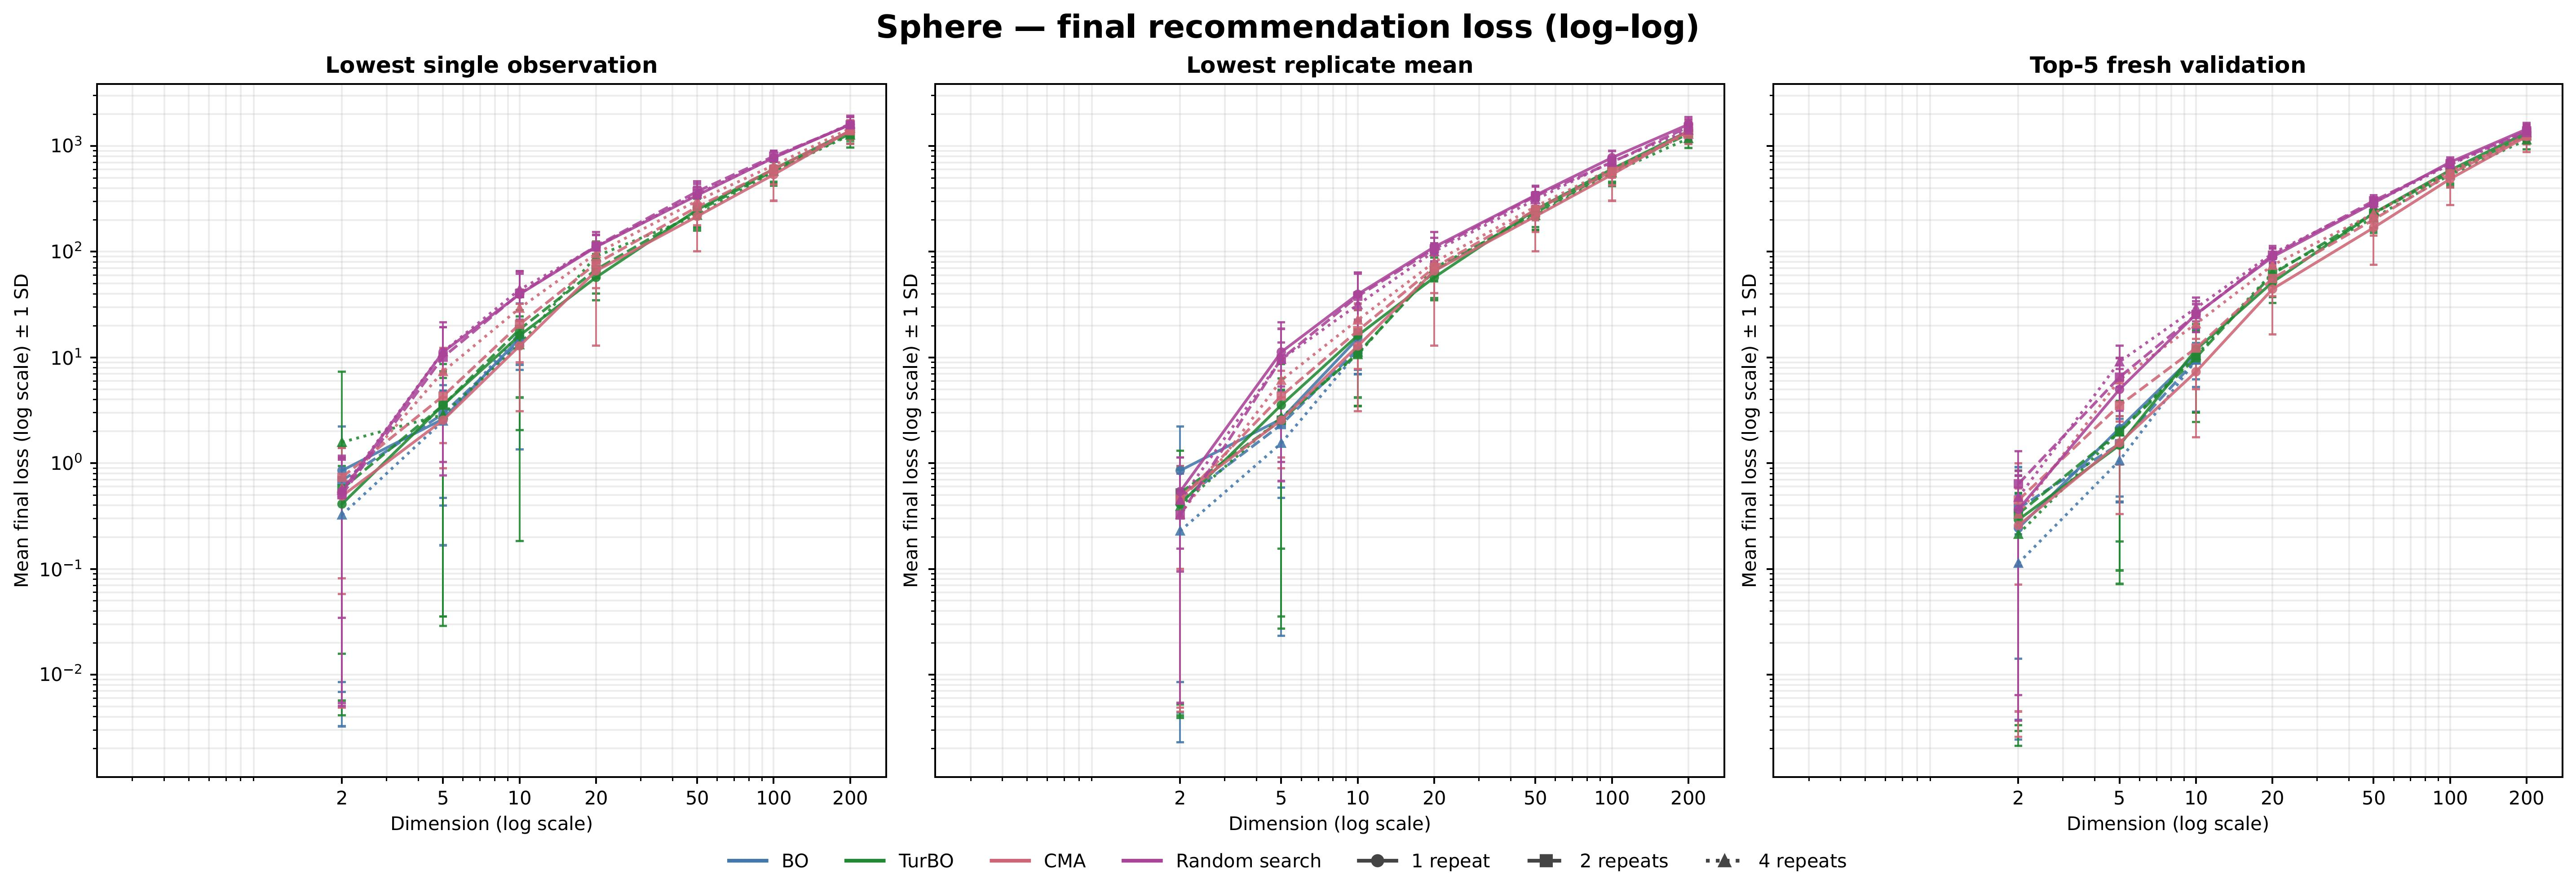
\includegraphics[width=0.8\textwidth]{loss_vs_dimension_loglog-images-0.png}
    \caption{Log-log plot of loss against Dimension for Sphere Function}
    \label{Sphere loss exp1}
\end{figure}
\begin{figure}[htbp]
    \centering
    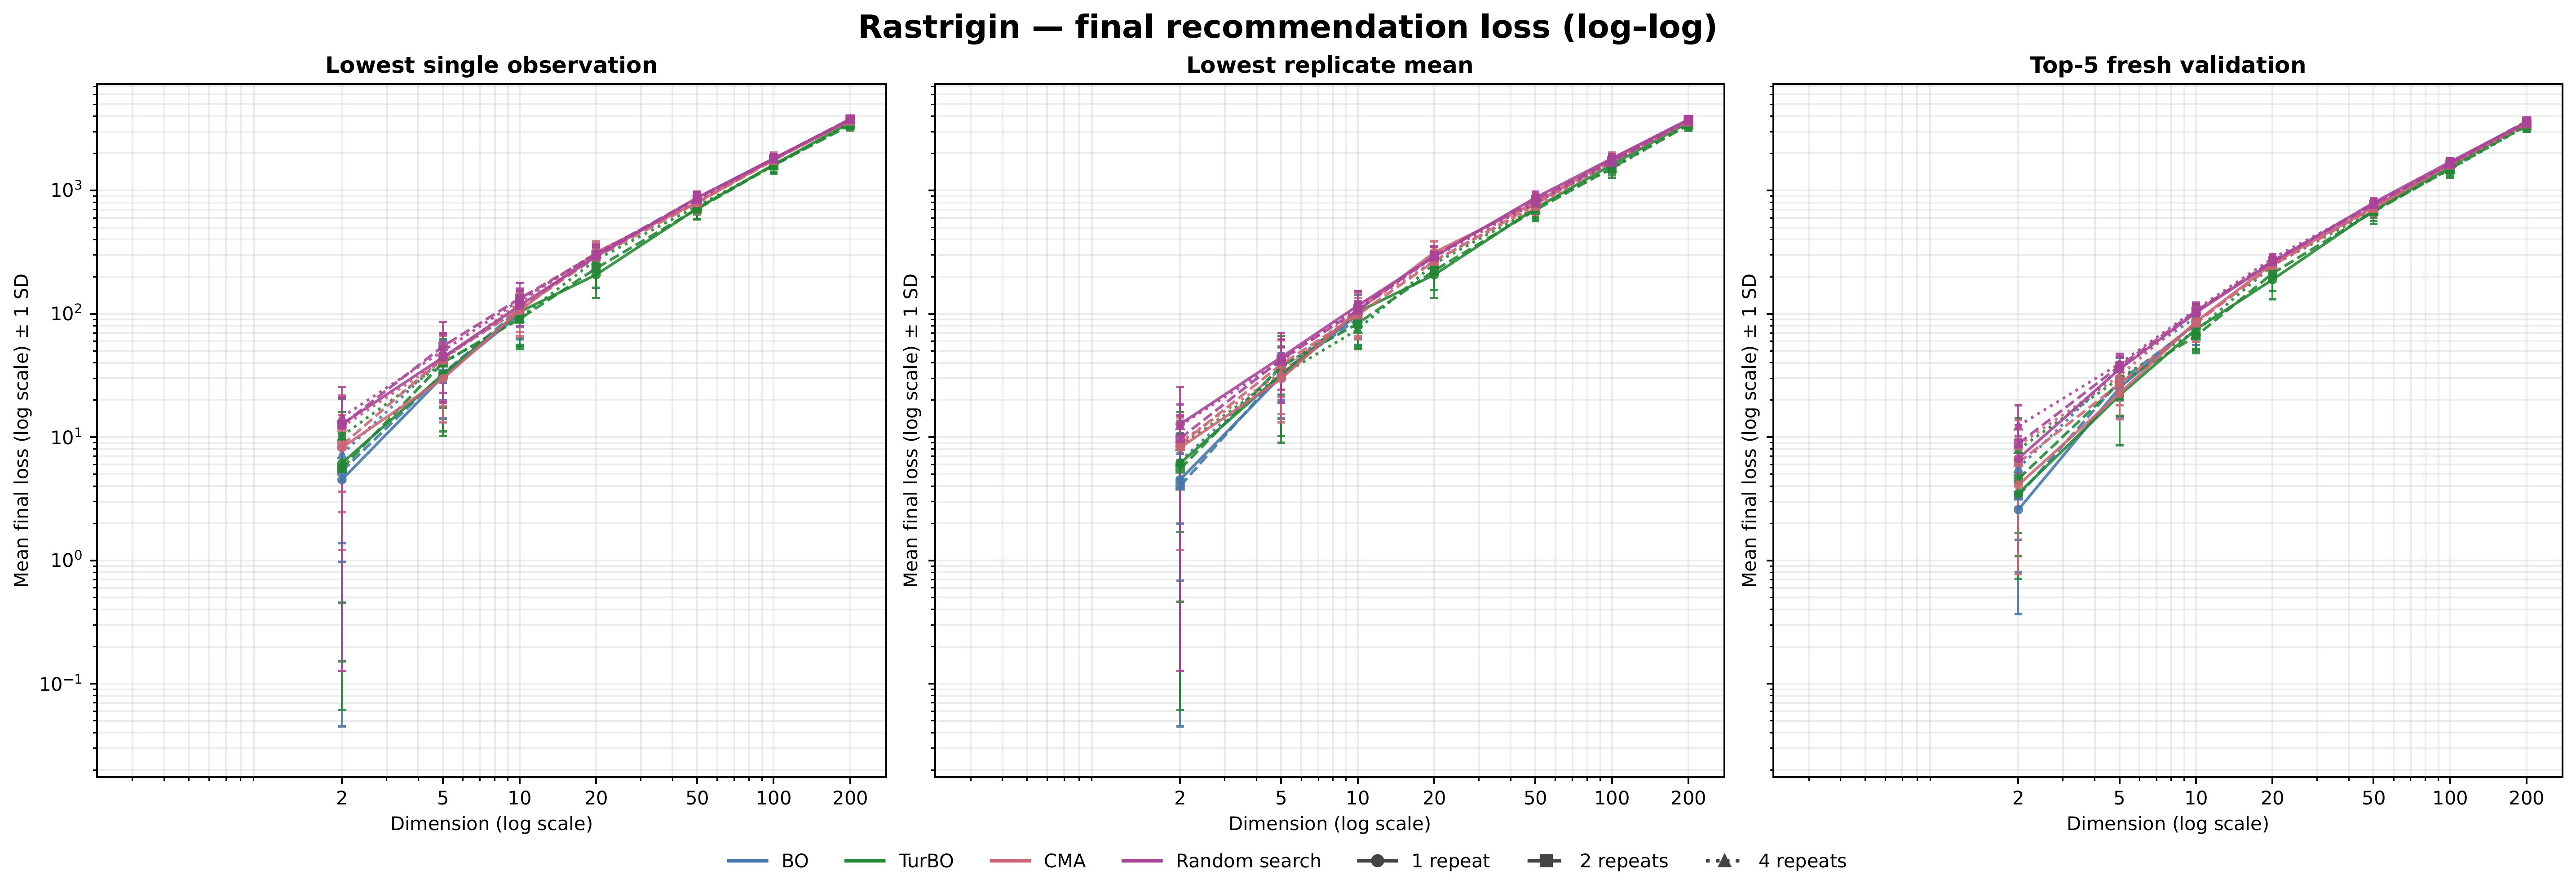
\includegraphics[width=0.8\textwidth]{loss_vs_dimension_loglog-images-1.png}
    \caption{Log-log plot of loss against Dimension for Rastrigin Function}
    \label{Rast loss exp1}
\end{figure}

We notice that while informed searches perform better than a random search, the results losses of all methods fall within 1 standard deviation of each other. This lack of meaningful improvement can be attributed to a small budget. Nonetheless, we can infer that across all three algorithms, the effect of spending more budget on repeat evaluations seems to reduce the losses in the case of the sphere, but increase losses in the case Rastrigin, the effect is more pronounced at low dimensions. This is likely because the sphere only has one global minimum with relatively simpler loss profiles. Hence more accurate evaluation would produce a model which more accurately fits the loss profile. However, for the Rastrigin function, the loss profile is more difficult to predict from just a local minimum, so more budget should be given to explore other sinks.

\begin{figure}[htbp]
    \centering
    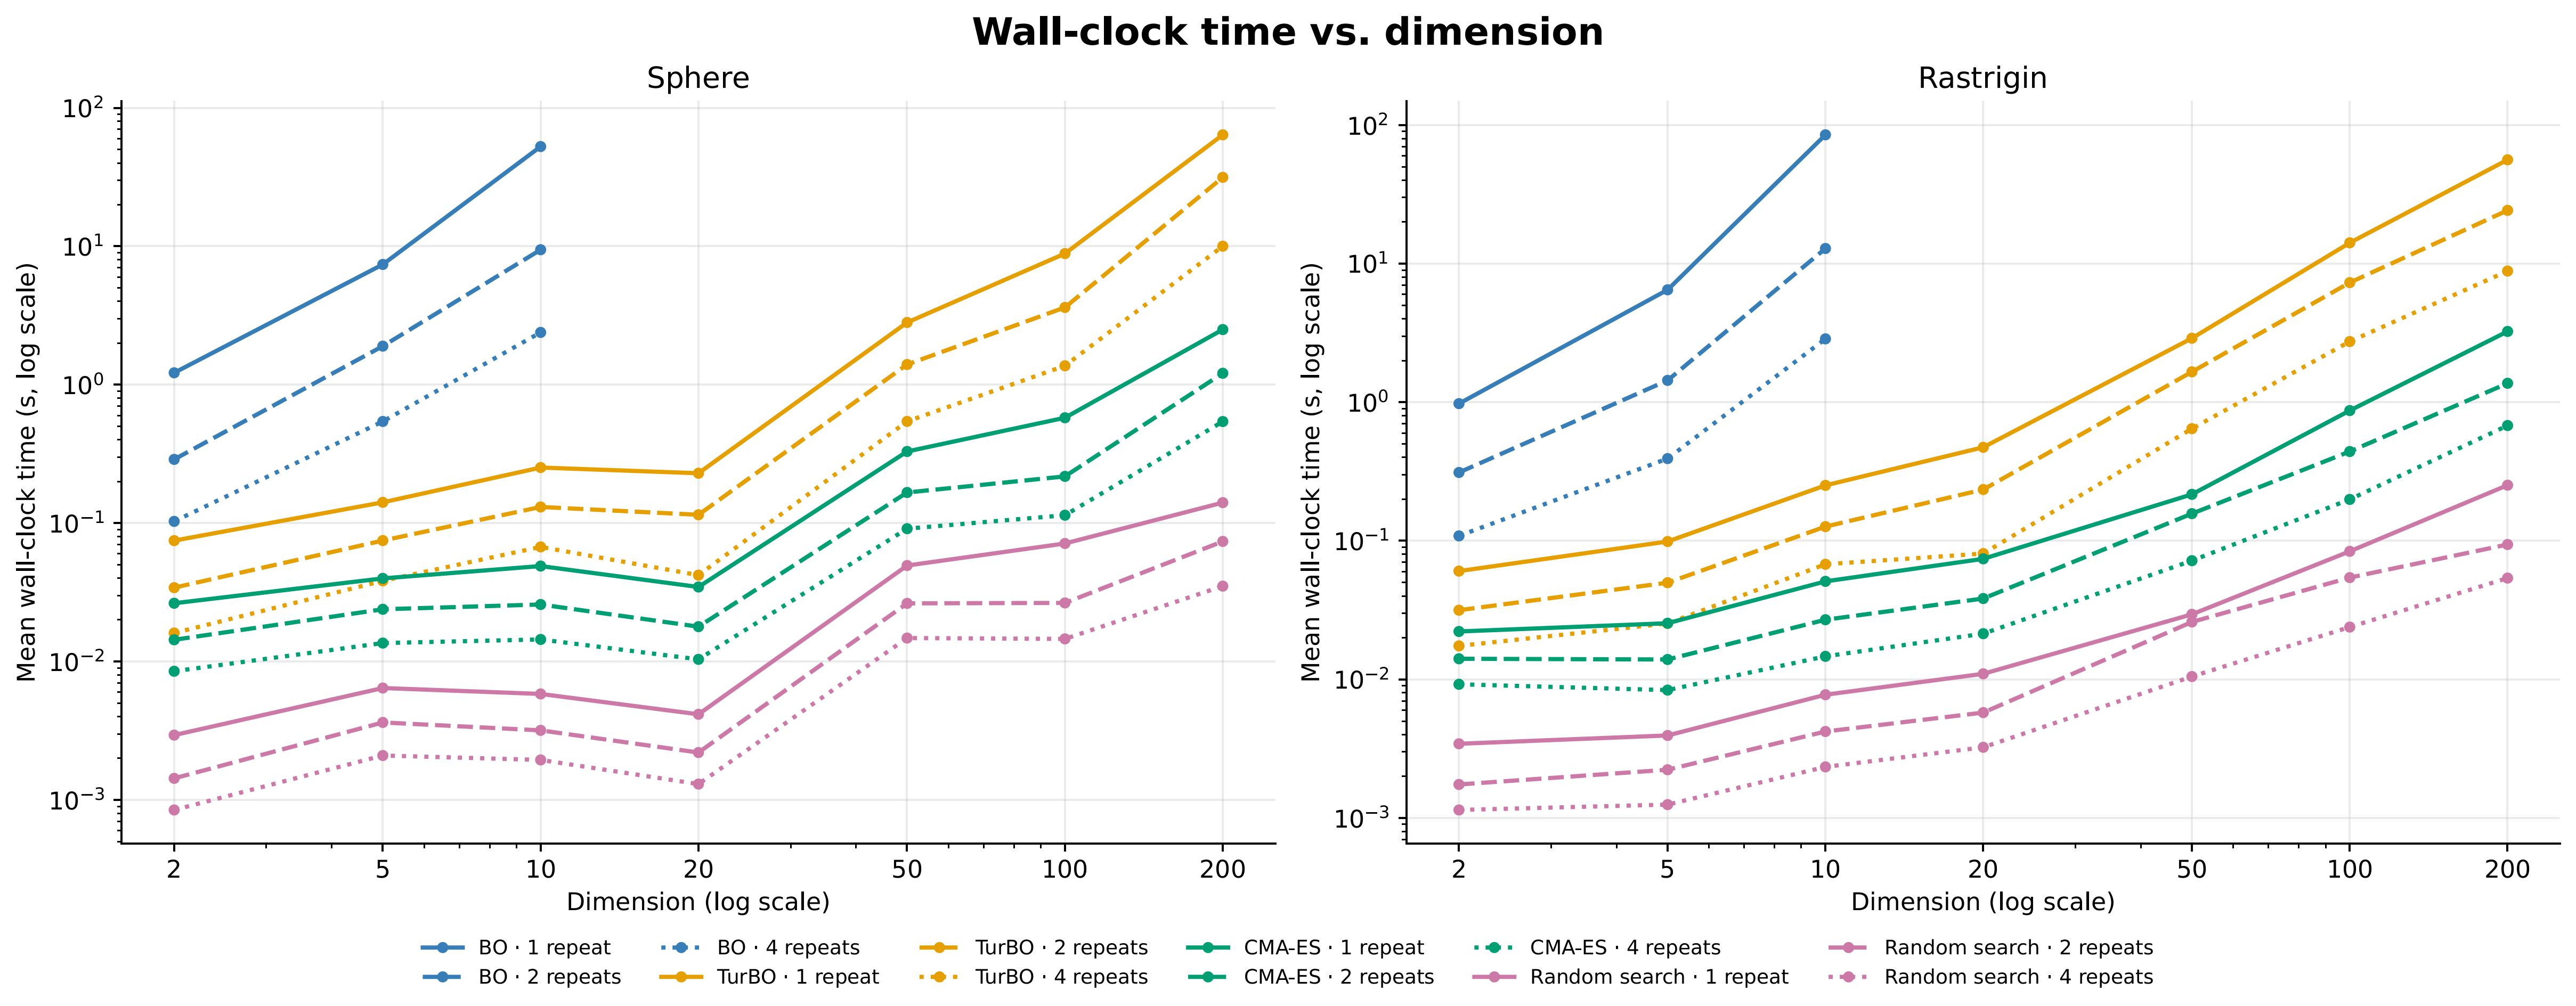
\includegraphics[width=0.8\textwidth]{wall_clock_time_loglog_simplified.jpg}
    \caption{Real Time Comparison}
    \label{Sphere loss exp1}
\end{figure}

In the case of $d \geq 20$, BO experiments exceeded the time allocated to run to completion. This shows that while BO generally is more accurate that TurBO and CMA in the case of low dimensions, it may not be feasible to optimize using BO for large dimensional spaces with the same evaluation budget and the same run-time budget. It is also clear that CMA generally performs faster than TurBo. This could be due to difficulty in expanding the trust area quick enough to capture a global minimum. Also spending more of the budget on repeat evaluations is faster than updating and recomputing the local/global gaussian distributions, which can be seen from the time taken for all four algorithms\footnote{Exact runtimes may defer depending on the machine used}.\\

Next, Fig. \ref{fig:side_by_side} shows the results the multi-modality test on 30 repeats of each algorithm. In the case of TurBO and BO, the results from different parameters are aggregated. For a parameter-level breakdown, see Fig. \ref{param side by side}. At the algorithm level, BO and TuRBO are consistently good performers in getting us closer (in $L^\infty$-distance) to the global optimum compared to CMA for the Ackley and Narrow Basin functions. All algorithms struggle against the Rastrigin function, espeically at $d=5$, although looking at the mean final distance, BO seems to perform slightly better than CMA, which performs slightly better than TuRBO. Also, on the Ackley function, TuRBO has the strongest performance with a distance success rate of $83\%$. It is also interesting to note that a random search seems to outperform all informed search algorithms at $d = 5$. This could be because adaptive local searches can struggle when the global optimum is distant from the initial search region, while random search focuses all of its computation on exploring the global region uniformly, meaning it is more likely to encounter a narrow global minima than informed search algorithms, which constructs a surrogate model using mostly flat local landscapes, hence concentrates most of its searches in a small area. In $d=2$, the number of evaluations needed before the search region or trust region adapts and moves to a more promising location is relatively lower so in most experiments, informed searches can still perform better within the allocated budget than a random search.\\

If we breakdown by algorithms, we can see that using improvement (EI, PI) as acquisition function dramatically increases the global basin success rate compared to UCB($13\%$). This could have been due to poor parameter tuning, for instance the choice of exploration parameter $\kappa = 2$ was fixed in all runs. It is likely that a larger choice of $\kappa$ would encourage more exploration and hence increase basin discoverability rate. For CMA runs, the best choice of population size is $2d$. In dimension $2$, 2 restart had more successes than the no-restart runs while the results are flipped in $d=5$. This suggests that with low budget, maintaining one sufficiently long CMA run can be more beneficial than repeatedly restarting before its search distribution has converged. In $d=2$, the size of the domain is relatively small for the budget and hence CMA can afford multiple restarts. This is not the case in $d=5$.\\
\begin{figure}[htbp]
    \centering
    \begin{subfigure}[b]{0.48\textwidth}
        \centering
        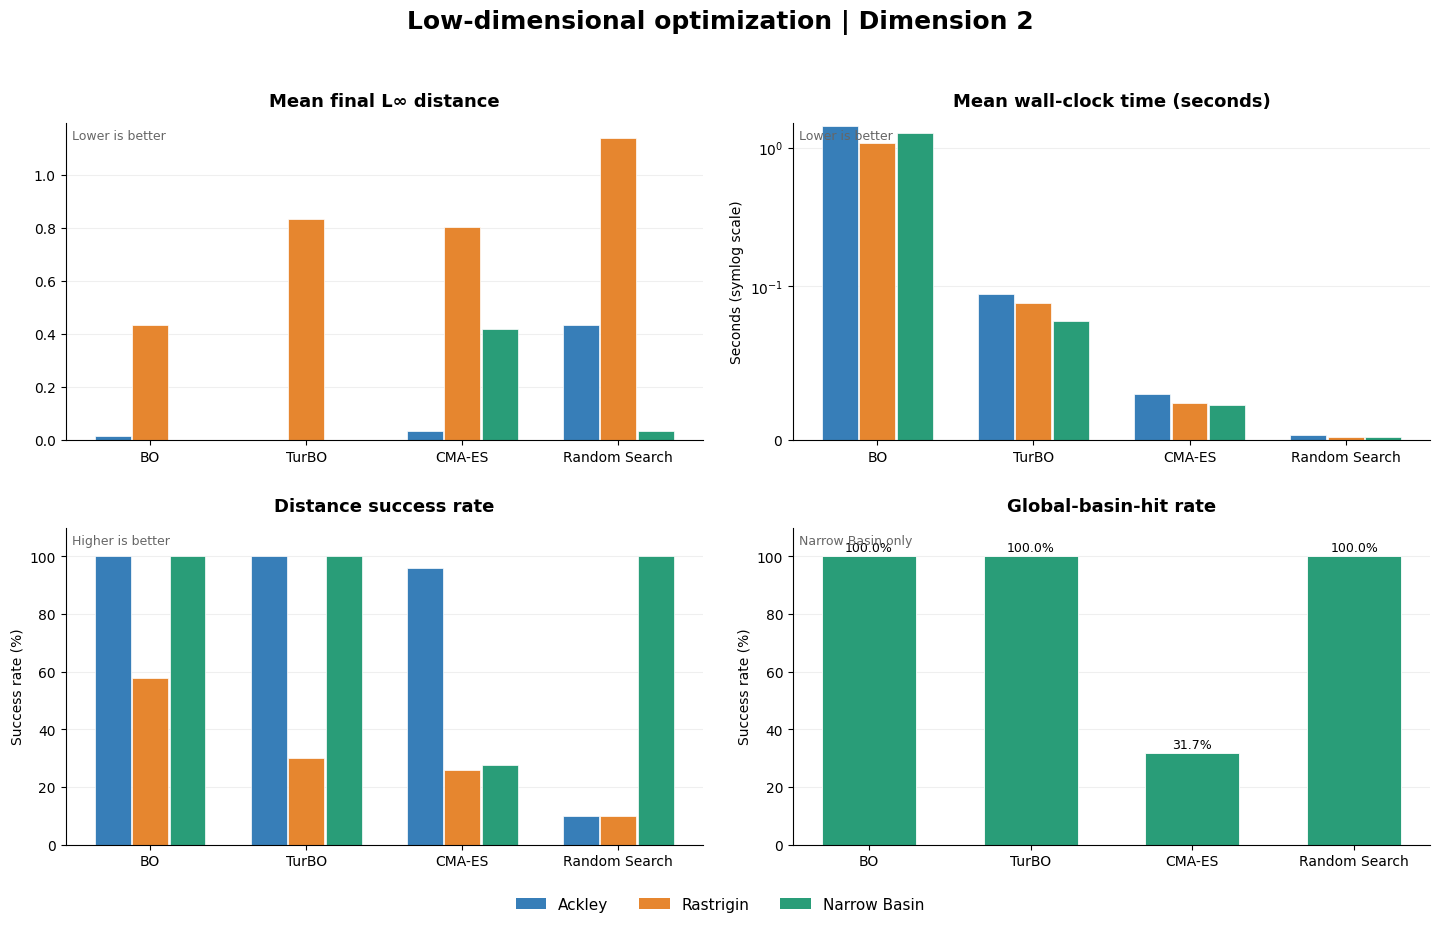
\includegraphics[width=\textwidth]{experiment2_dim2_algo_level.png}
    \end{subfigure}
    \hfill % Adds horizontal space between the two subfigures
    \begin{subfigure}[b]{0.48\textwidth}
        \centering
        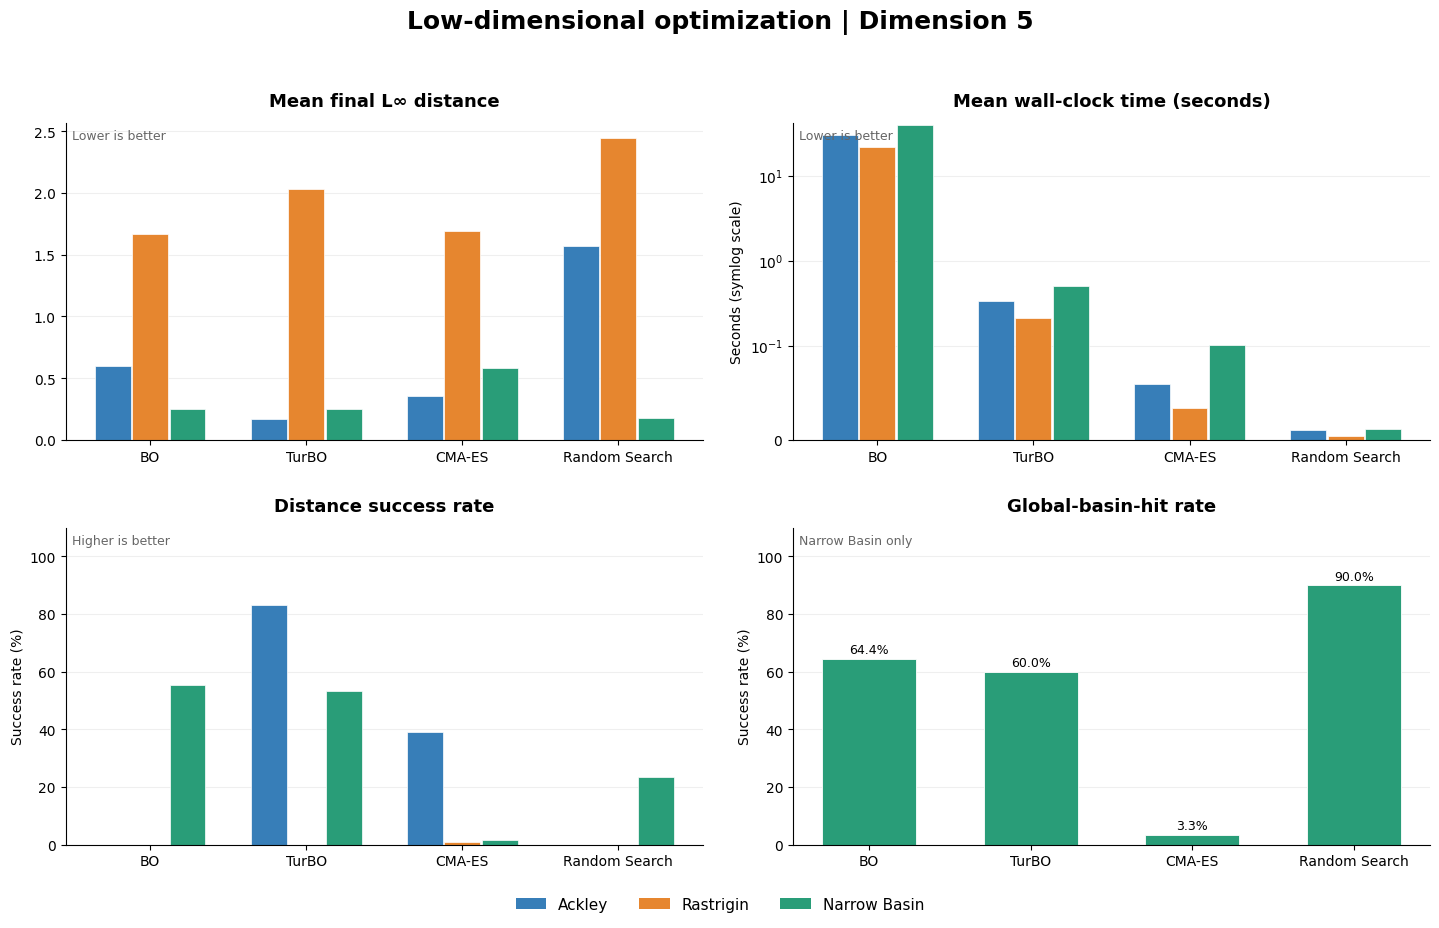
\includegraphics[width=\textwidth]{experiment2_dim5_algo_level.png}
    \end{subfigure}
    \caption{Small Dimension Multi-modality Performance (Algorithm Level)}
    \label{fig:side_by_side}
\end{figure}
For larger dimension runs, as before we shall not consider naive BO due to time complexity. Fig. \ref{large dimension 2} shows that the CMA with population $100d$ and no restarts performs the best on the Ackley function. A look at the loss profiles (Fig. \ref{losses side by side}) explains why. The same seed produces the same initial convergence path for CMA (pop = $200$), however, with restarts, the convergence is terminated too early before the algorithm looks for another starting point, causing the plateau of the best so far graph for CMA with restarts, while the CMA without restarts is given the remaining two-thirds of the budget to converge. TURBO on the other hand is able to discover the basin within one-tenth of the evaluation budget but then progress stalls. This is likely due to the many ripples near the global minimum which causes the trust region to expand unnecessarily even though in actually fact the points are already close to the global minimum. This means convergence will be much slower as the algorithm is incentivised to look for points far away from where it already it (near the minimum).\\
\begin{figure}[htbp]
    \centering
    \begin{subfigure}[b]{0.48\textwidth}
        \centering
        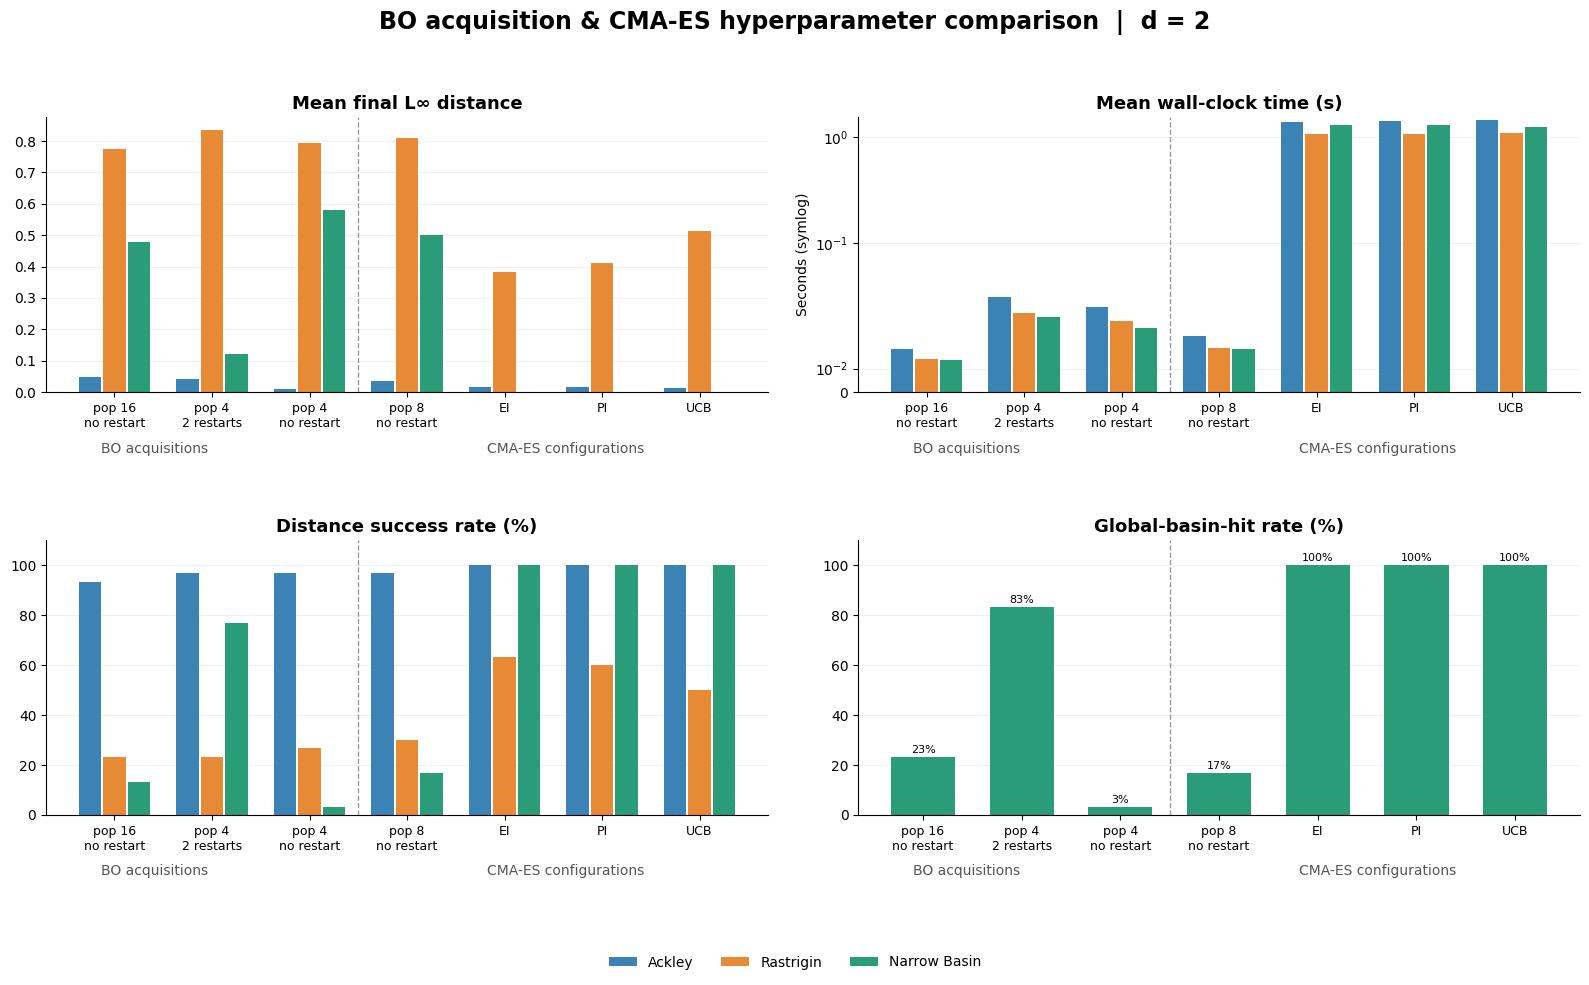
\includegraphics[width=\textwidth]{parameter_level_exp2_dim2.png}
    \end{subfigure}
    \hfill % Adds horizontal space between the two subfigures
    \begin{subfigure}[b]{0.48\textwidth}
        \centering
        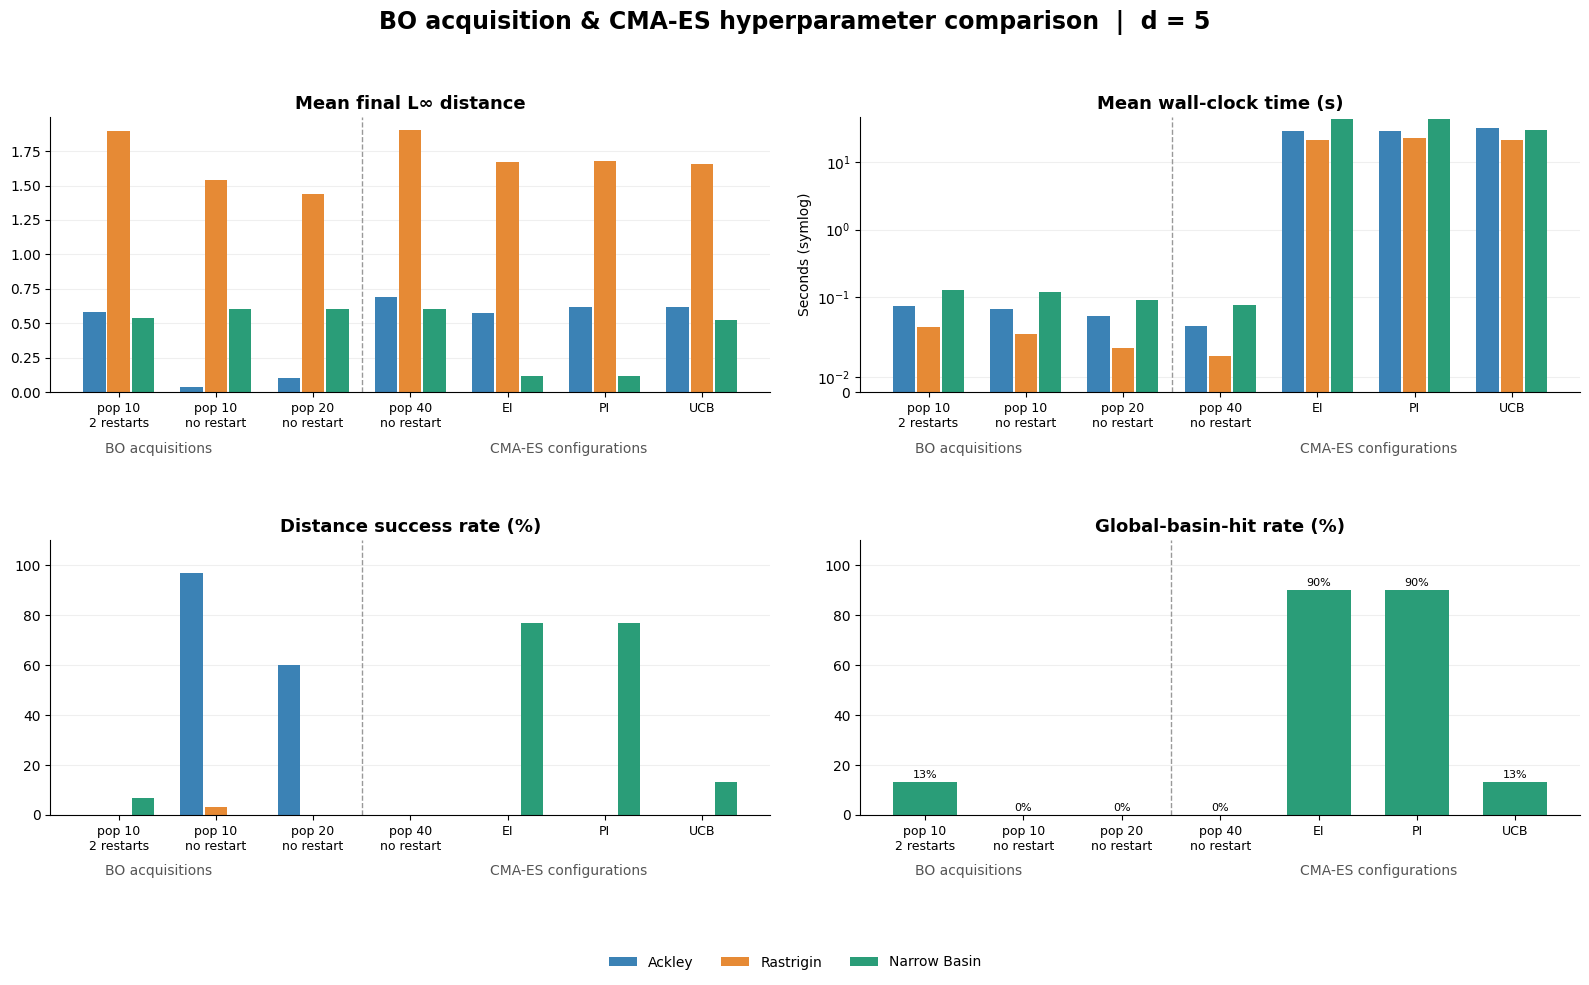
\includegraphics[width=\textwidth]{parameter_level_exp2_dim5.png}
    \end{subfigure}
    \caption{Small Dimension Multi-modality Performance (Parameter Level)}
    \label{param side by side}
\end{figure}
These results suggest that the best algorithm depends on the nature of the multi-modality, as can be seen from the differing performances over different functions. CMA is robust against local ripples and performs very well in higher dimensions. On the other hand, TuRBO and BO tend to be slower but outperform CMA in low dimensional setting. This too however, is dependent on a good tuning of the exploration parameter.\\
\begin{figure}[htbp]
    \centering
    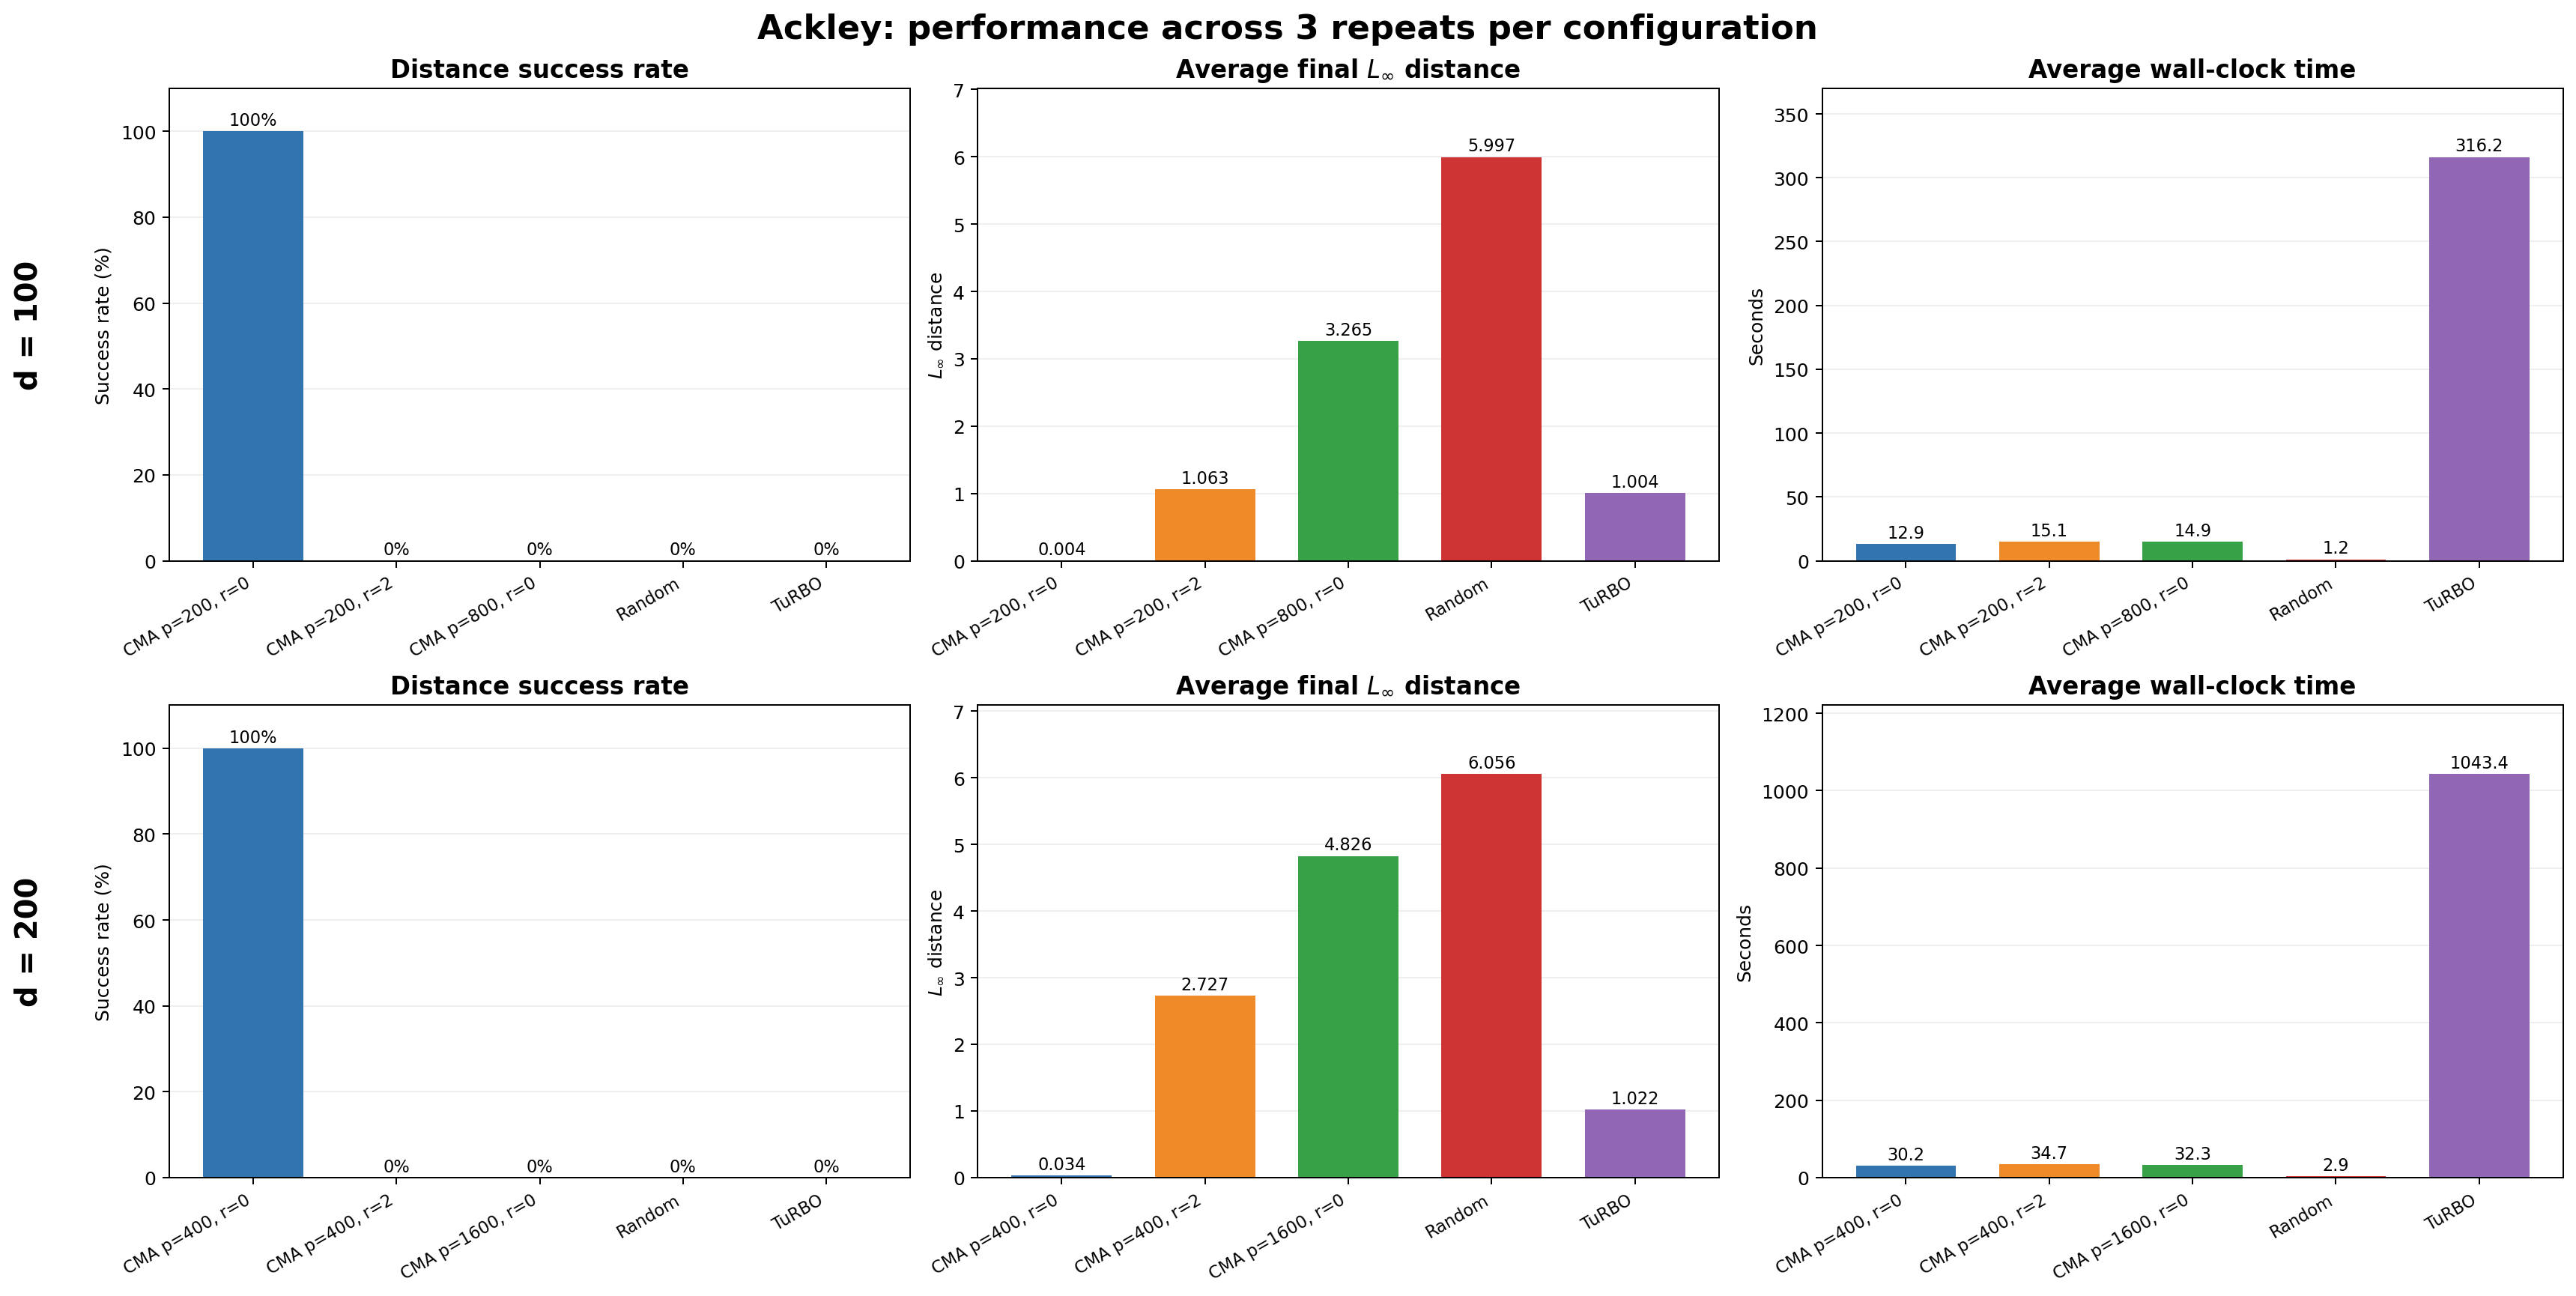
\includegraphics[width=0.8\textwidth]{exp2_large_combined_2x3.png}
    \caption{Large Dimension Multi-modality Performance}
    \label{large dimension 2}
\end{figure}

\begin{figure}[htbp]
    \centering
    \begin{subfigure}[b]{0.48\textwidth}
        \centering
        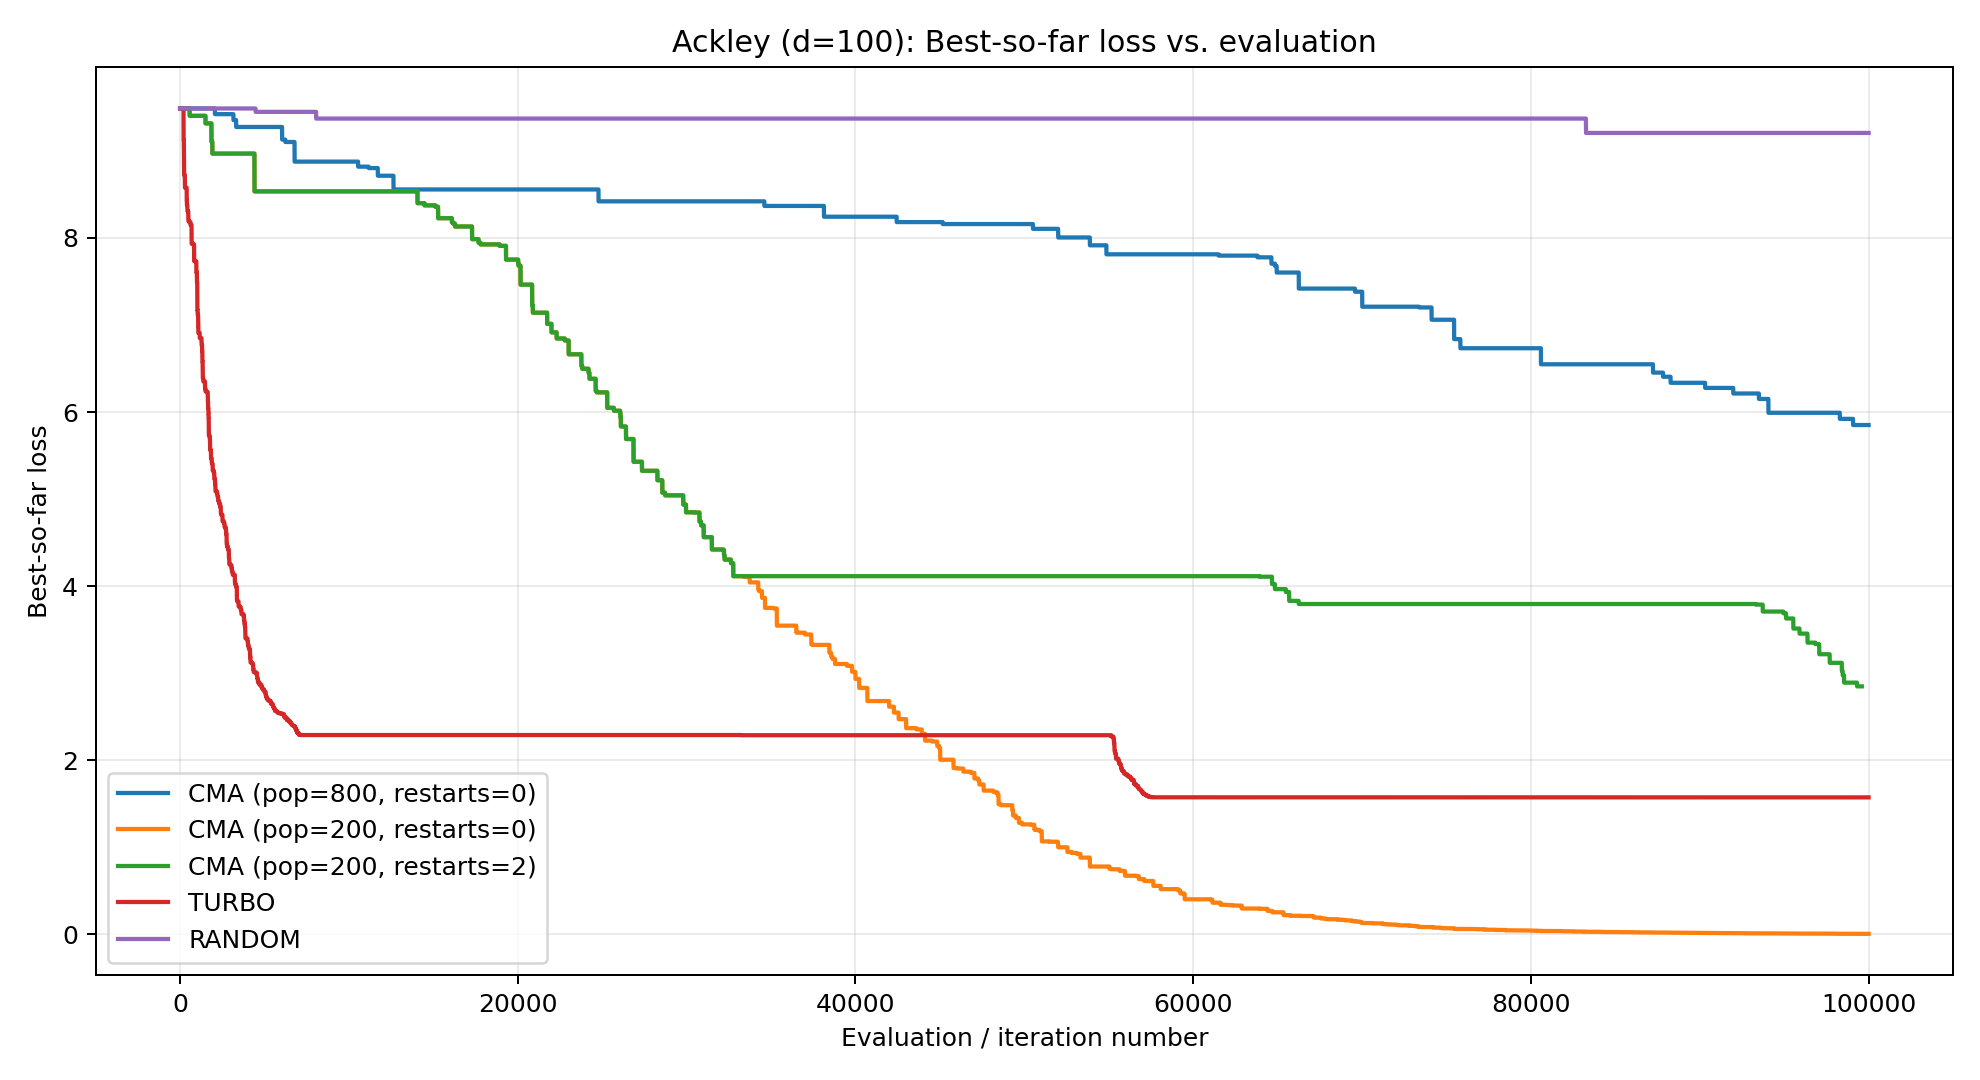
\includegraphics[width=\textwidth]{exp2_loss_profiles_dim_100.png}
    \end{subfigure}
    \hfill % Adds horizontal space between the two subfigures
    \begin{subfigure}[b]{0.48\textwidth}
        \centering
        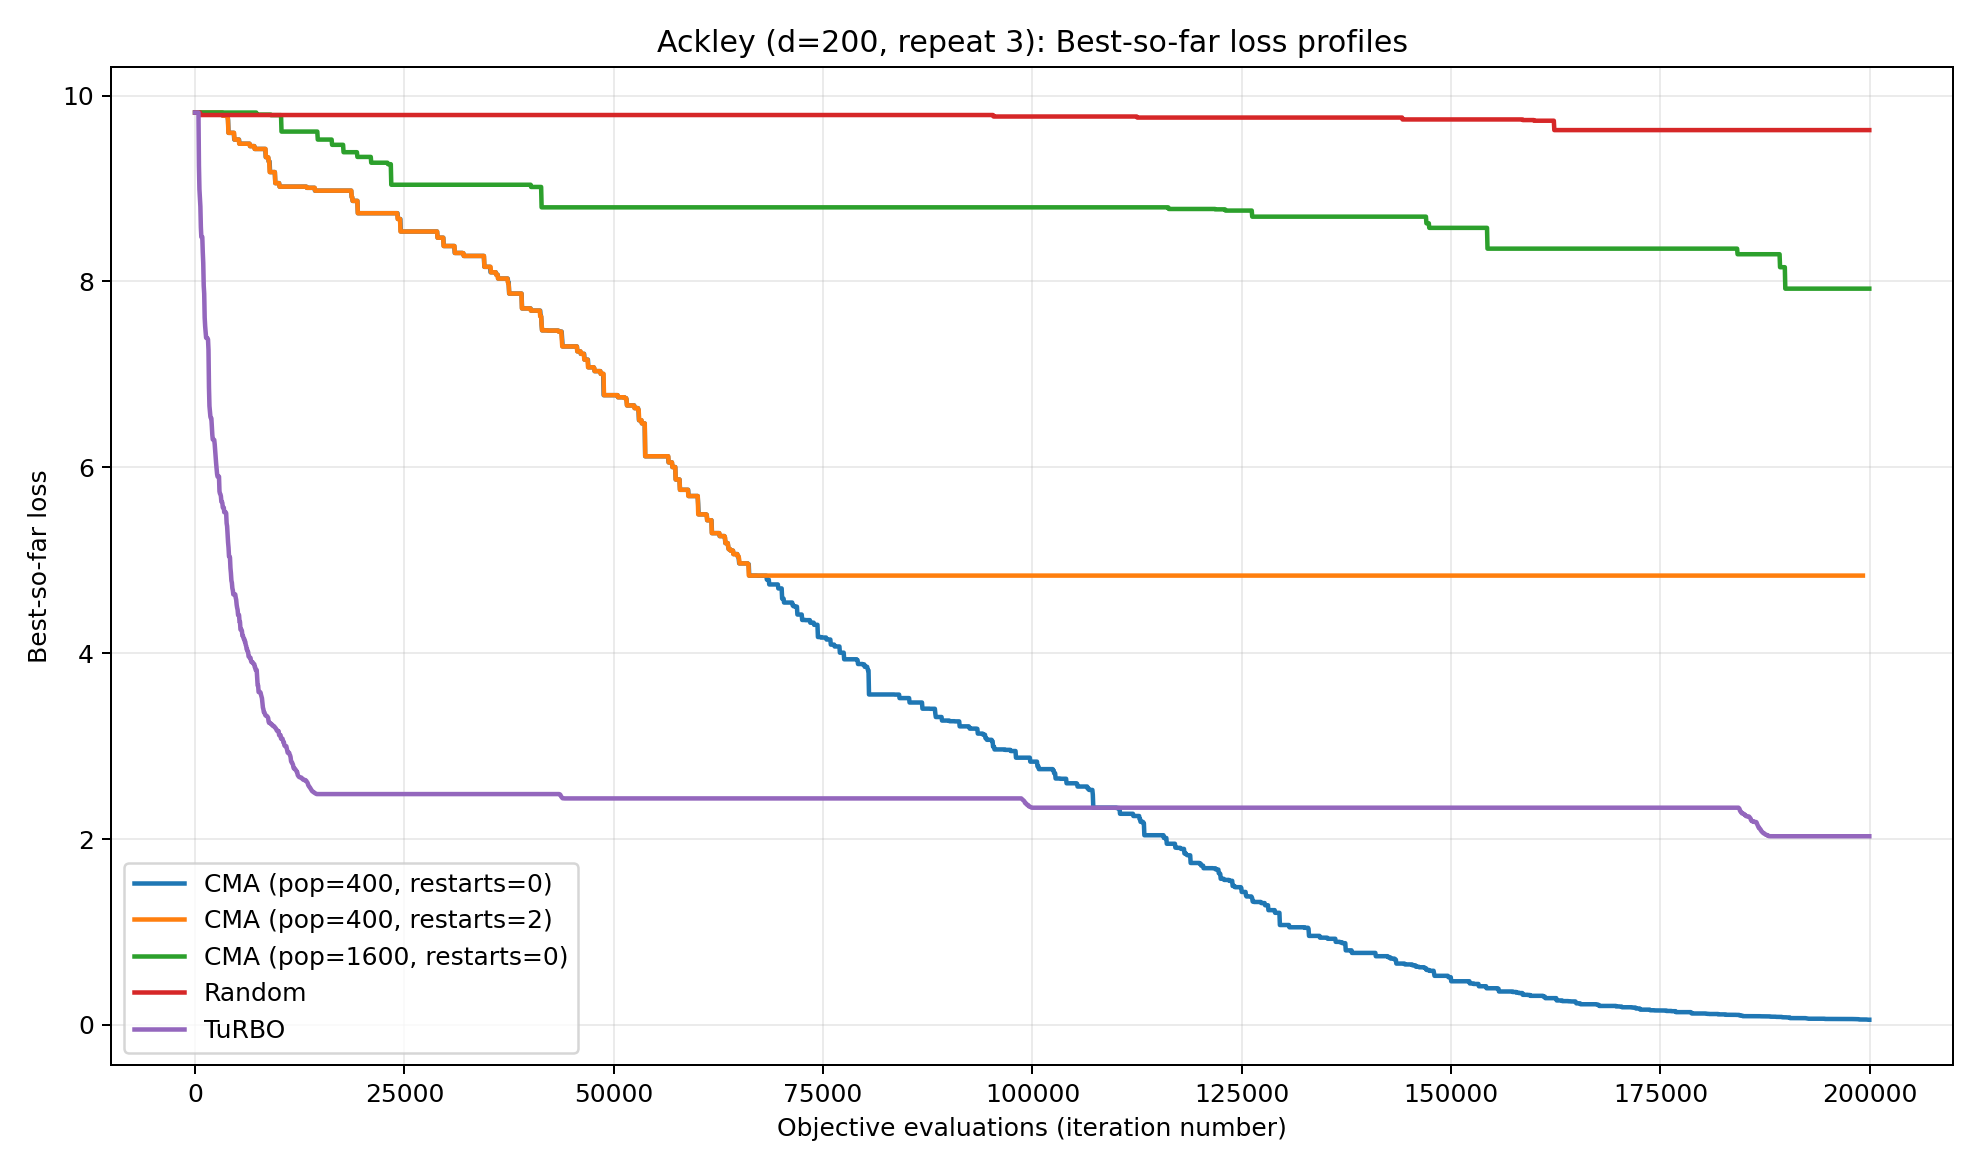
\includegraphics[width=\textwidth]{exp2_profiles_dim_200.png}
    \end{subfigure}
    \caption{Best-so-far Loss Profiles from One Run with Ackley at $d=100,200$}
    \label{losses side by side}
\end{figure}

\begin{figure}[htbp]
    \centering
    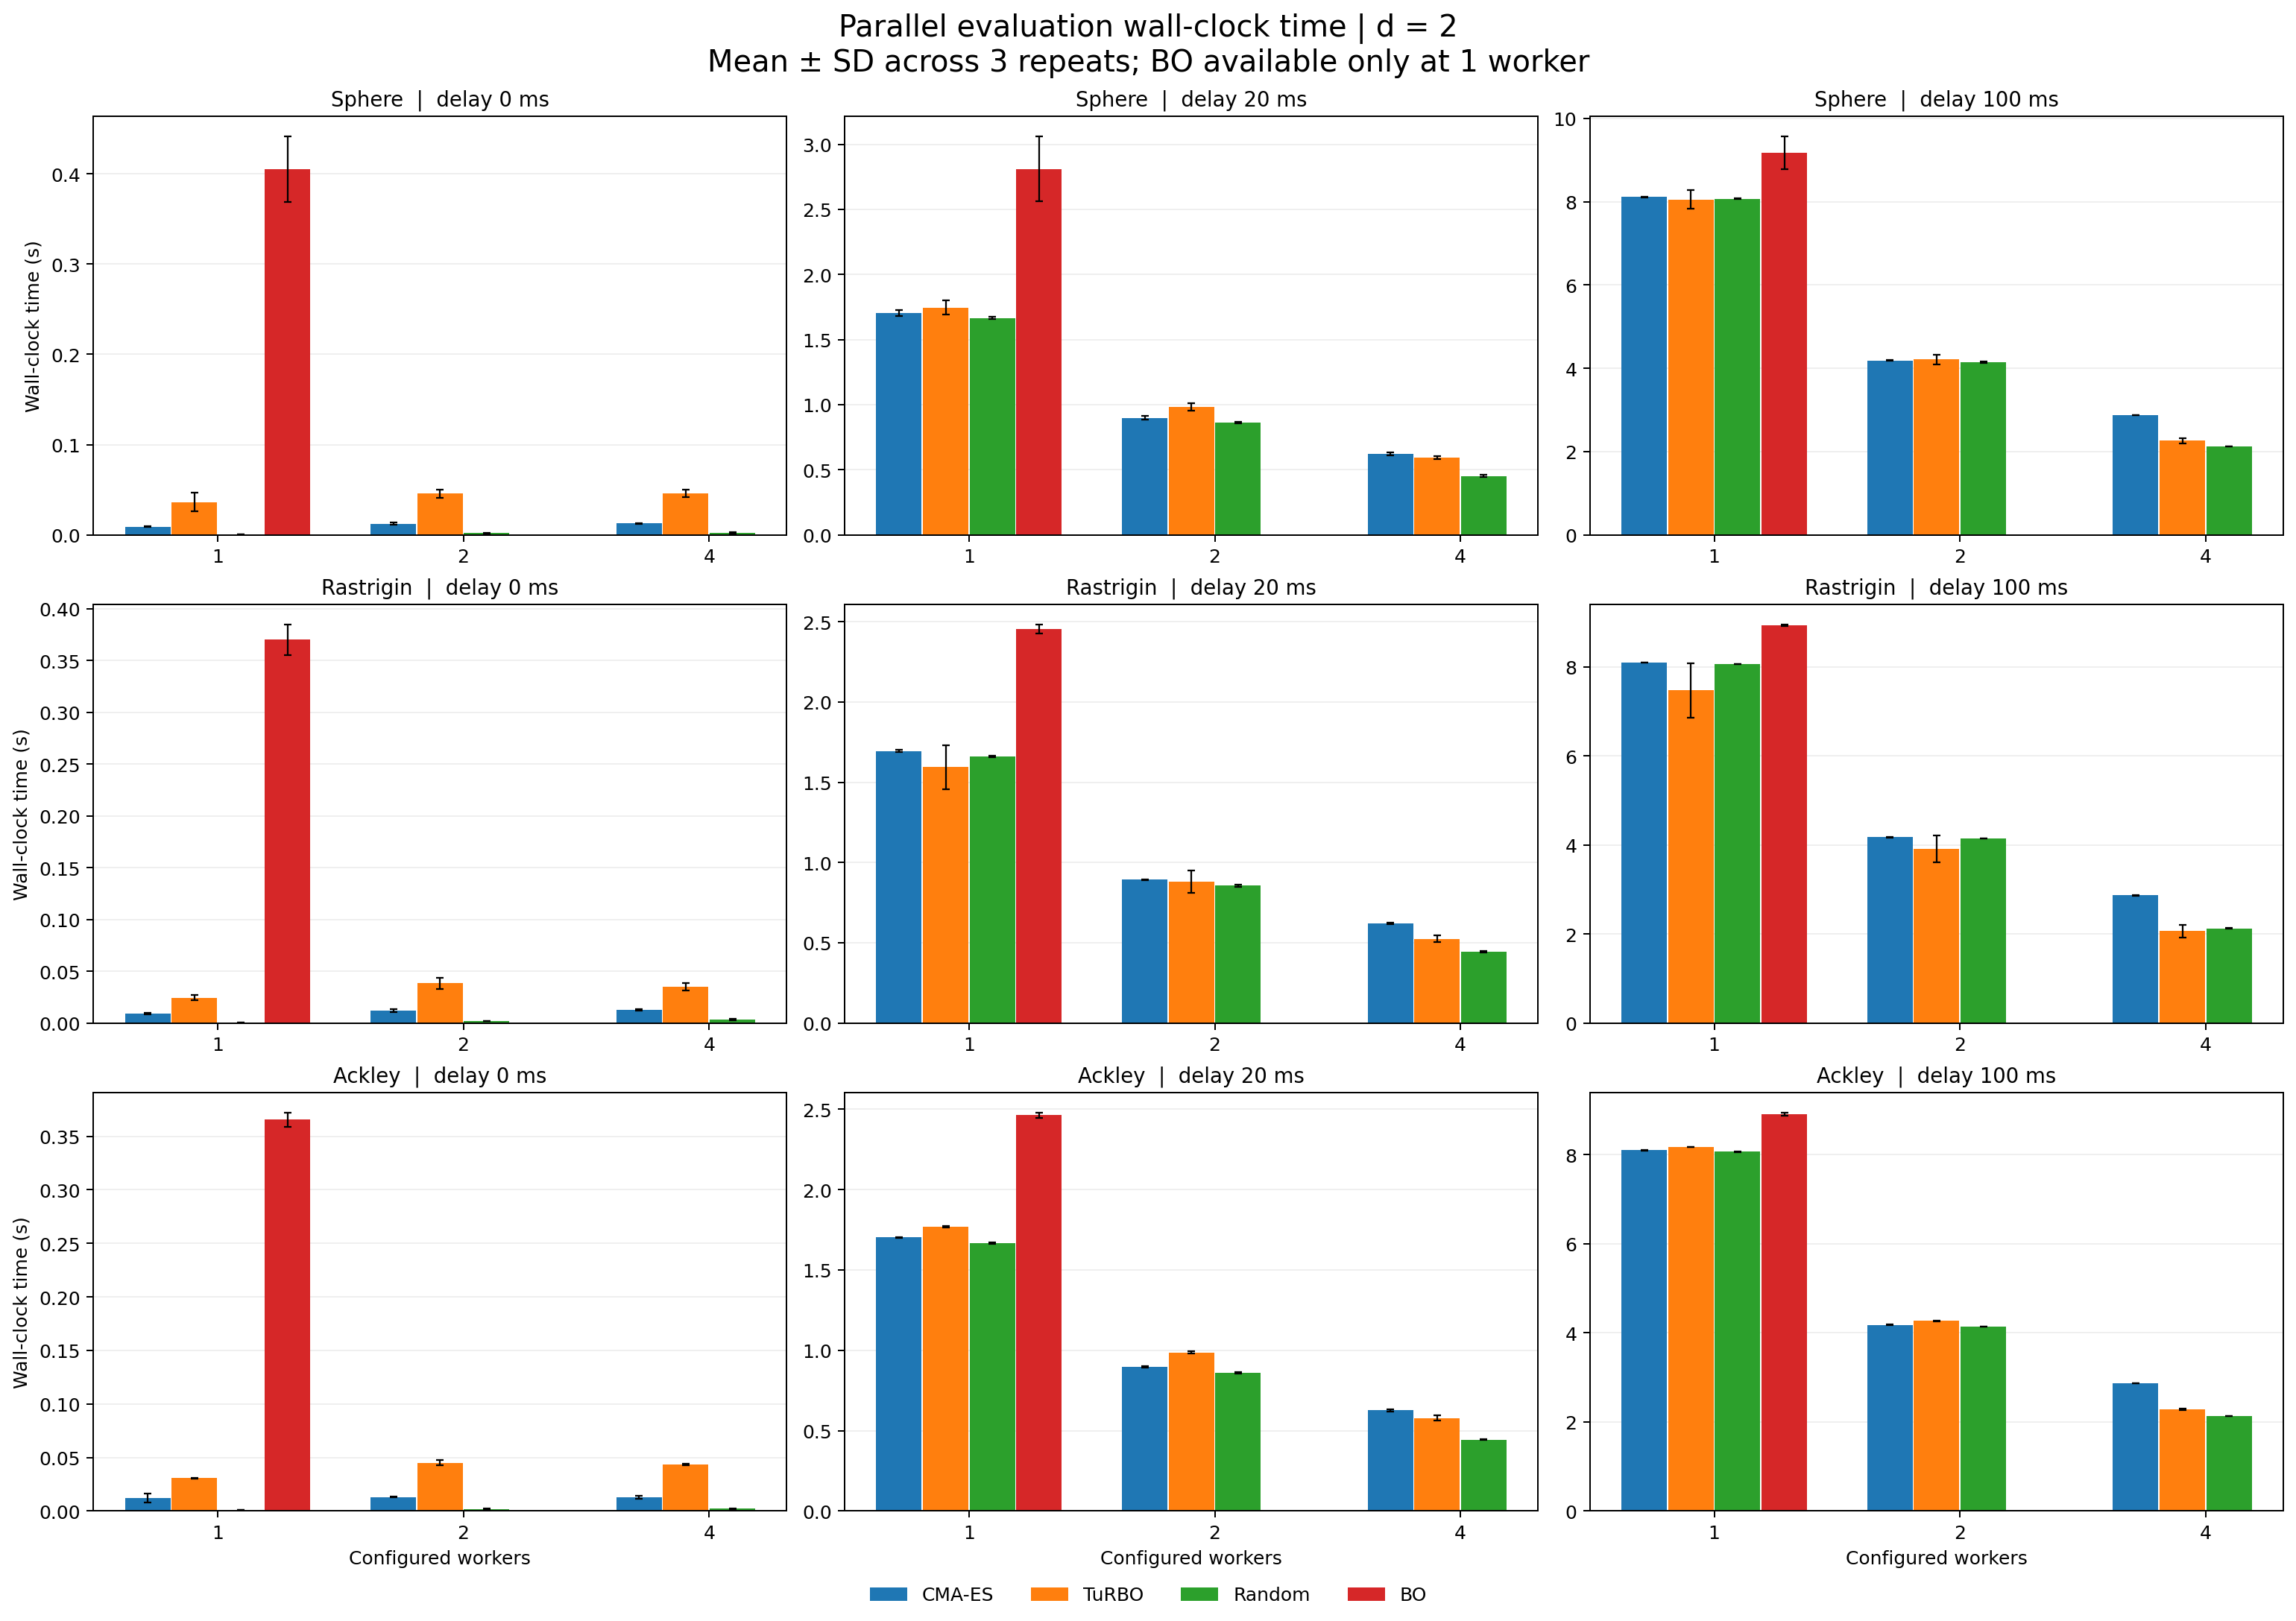
\includegraphics[width=0.8\textwidth]{exp3_d2.png}
    \caption{Effect of Adding Multiple Workers at $d=2$}
    \label{workers dim 2}
\end{figure}
\begin{figure}[htbp]
    \centering
    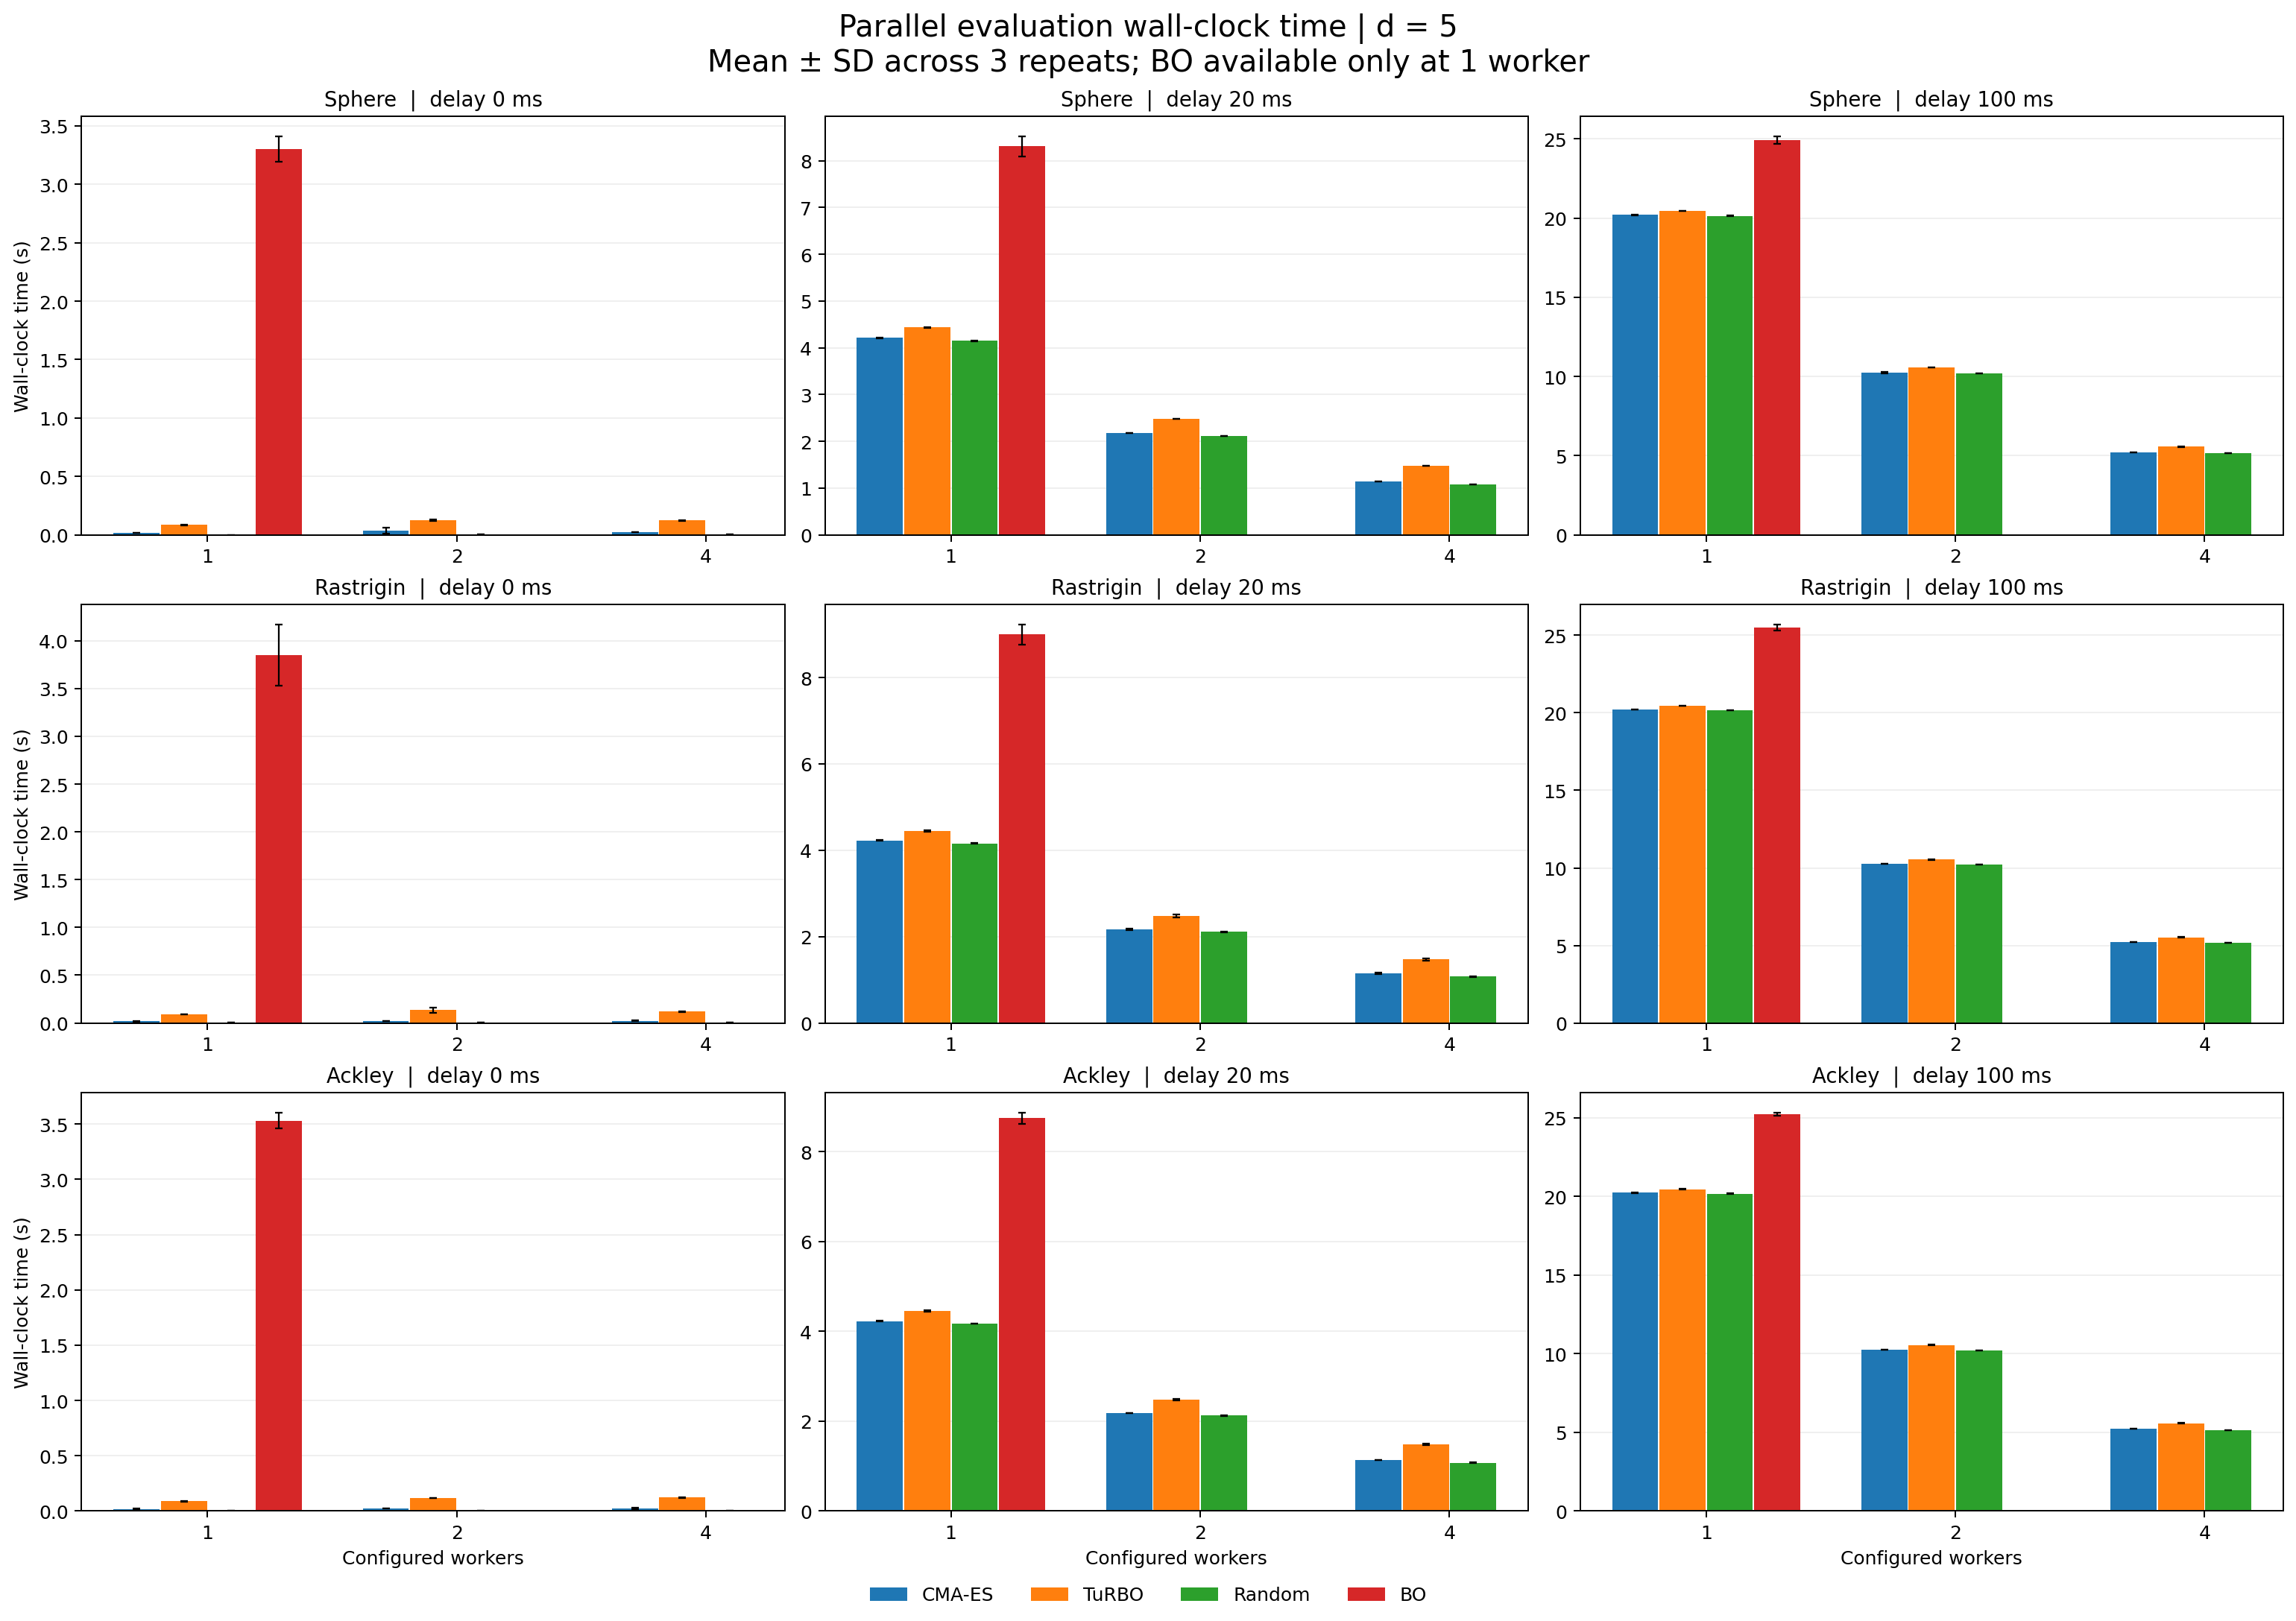
\includegraphics[width=0.8\textwidth]{exp3_d5.png}
    \caption{Effect of Adding Multiple Workers at $d=5$}
    \label{workers dim 5}
\end{figure}

Fig. \ref{workers dim 2} and \ref{workers dim 5} show the effect of adding multiple workers to the computation time. In the current implementation, adding workers produces very little overhead and hence is always more beneficial to run multiple computations in parallel for even small delays of $\geq 20ms$. It is possible that for delays smaller than $20ms$ or with more workers than $4$, the overhead becomes more significant relative to time savings.
\FloatBarrier
\section{Limitations}

The experiments rely primarily on  objective functions that are continuous and, for the most part, smooth. In other words, they have a small modulus of continuity. These functions may not adequately represent the complexity of real-world optimization problems, which can involve discontinuities, non-differentiability, constraints, and irregular or non-stationary objective landscapes. Secondly, the noise models considered are restricted to Gaussian and Student's $t$-distributed noise. These distributions are relatively easy to implement and quick to sample from (meaning they do not affect the actual run-time of each algorithm). This allows the characteristics of each algorithm to be studied under controlled conditions. However, real-world evaluation noise may exhibit more complicated properties, such as heteroscedasticity or time-dependence.These not captured by the models considered here.\\

Furthermore, the evaluation budgets and number of independent runs used in the experiments are limited. Consequently, the results may not fully reflect the algorithms' performance under larger evaluation budgets or provide a sufficiently comprehensive picture of their variability across different initial conditions and random seeds. The observed differences should therefore be interpreted within the experimental settings rather than as definitive rankings of the algorithms. Finally, the results are dependent on the specific implementations and parameter configurations used in this study, including choices of population size, restart policy, acquisition function, and trust-region parameters. Different implementations, hyperparameter settings, or optimization strategies may produce different outcomes. In particular, the findings regarding the relative performance of CMA, TuRBO, and BO should not be assumed to generalize to all implementations of these algorithms.

\section{Declaration}
Code and READme was written with the help of ChatGPT.
\begin{thebibliography}{9}

\bibitem{turboarticle} Eriksson, D., Pearce, M., Gardner, J. R., Turner, R., \& Matthias, P. (2019). Scalable global optimization via local bayesian optimization (1910.01739v4). arXiv. https://arxiv.org/abs/1910.01739v4

\bibitem{CMA} Nikolaus, H. (2016). The CMA evolution strategy: A tutorial (1604.00772v2). arXiv. https://arxiv.org/abs/1604.00772v2

\end{thebibliography}

\end{document}